\documentclass{article}

% Cabecera del documento
% ======================================================================

% Paquetes extras
\usepackage[square, numbers, sort]{natbib}
% \usepackage{cite}
\usepackage{graphicx}
\usepackage[utf8]{inputenc}
\usepackage{amsmath,amssymb,amsfonts}
\usepackage{algorithmic}
\usepackage{textcomp}
\usepackage{subfig}
\usepackage{float}
\usepackage{mathtools}
\usepackage[spanish]{babel}
\usepackage[paper=a4paper,margin=2.75cm]{geometry}
\usepackage{booktabs} % for tables
\usepackage[colorlinks = true,
            linkcolor = blue,
            urlcolor  = blue,
            citecolor = orange,
            anchorcolor = blue]{hyperref} % for hyperlinks
\usepackage{xcolor} % text colors
\usepackage{minted}


% Directorio con imagenes
\graphicspath{{./figs/}}

% Cabecera del documento
% ======================================================================

% Titulo
\title{\textbf{CONTROL DE LA PRIMER ARTICULACIÓN DE ROBOT SERIE DE SEIS GRADOS DE LIBERTAD}}

% Autores
\author{Rodrigo Pérez \\ rodrigoperez2110@gmail.com \\ \\ Control y Sistemas, Facultad de Ingeniería, \\ Universidad Nacional de Cuyo, \\ Mendoza, Argentina}

% Fecha
\date{Febrero de 2024}

% Cuerpo del documento
% ======================================================================
\begin{document}

% Comandos definidos por el autor
\renewcommand{\tablename}{Tabla}
% \renewcommand{\color{blue}{#1}}{\azul}

% Crear cabecera
\maketitle


\begin{figure}[H]
    \centering
    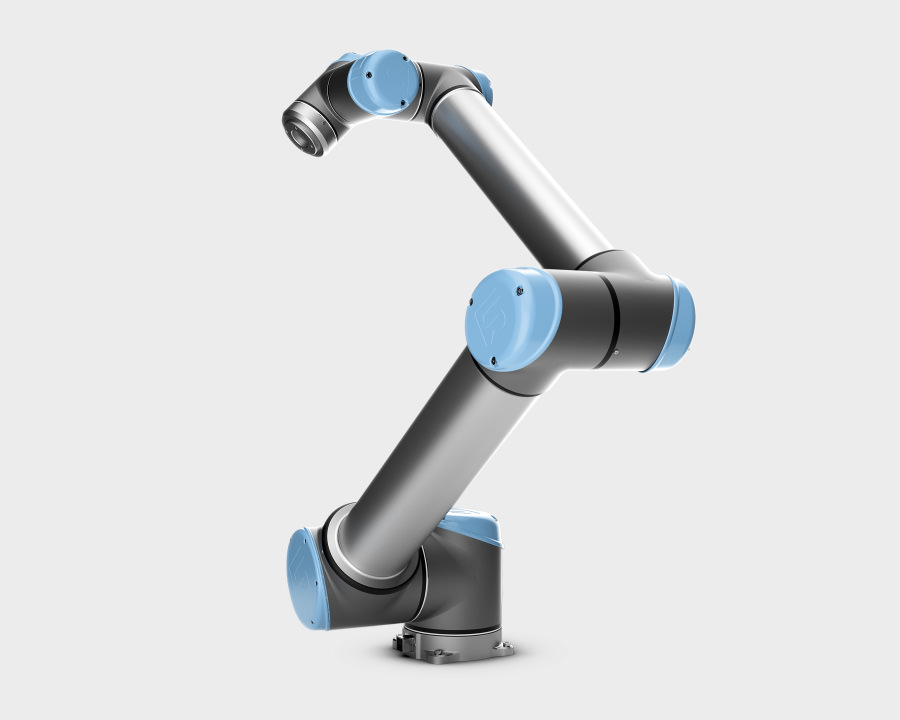
\includegraphics[width=1\textwidth]{UR10-UNIVERSAL-ROBOT}
    \caption{Robot Universal UR10}
    \label{fig:UR10-UNIVERSAL-ROBOT}
\end{figure}


% Resumen
% ======================================================================
\begin{abstract}
    El presente documento presenta el proyecto final de la cátedra de Control y Sistemas de la Universidad Nacional de Cuyo.
    El OBJETIVO del proyecto es aplicar los conocimientos, herramientas y habilidaddes adquiridas para realizar el análisis, modelado y simulación del control de posición para el accionamiento electromecánico de la primer articulación del robot Universal UR10 figura \ref{fig:UR10-UNIVERSAL-ROBOT}, un robot industrial tipo serie de 6 grados de libertad.

    El robot se modela como un Sistema Lineal Variante en el Tiempo, en donde se toma al momento de inercia como un parámetro variable, y se utiliza un tipo de Controlador PID aplicado con la técnica de Gain Schedule.

    Además, se incluye el modelado de un sensor ruidoso a la salida del sistema, se usa un filtro anti-aliasing y se propone un filtrado adicional con el objetivo de mitigar el ruido.

    Luego, se valida el modelo mediante la comparación con otro modelo ("más realista") del sistema, el Modelo de Validación; el cual incluye las No Linealidades del robot, y en en el cual se utiliza un Controlador Discreto con Representación en Punto Fijo. El controlador se diseña en tiempo continuo, como se trabajó durante el cursado, pero en el modelo de validación, el bloque del controlador se implementa en tiempo discreto y punto fijo. ["Todo hecho en Simulink"].

\end{abstract}


% Secciones
% ======================================================================


\section{INTRODUCCIÓN}
\label{sec:INTRODUCCIÓN}

Los brazos robóticos de varios eslabones en serie, llamados robots serie, poseen un Subsistema Mecánico Fuertemente No Lineal. Esto es debido a que, para cada articulación del robot, la posición (y también la velocidad y aceleración) de las demás articulaciones influyen en su dinámica.
Por otro lado, un controlador PID es una técnica de control lineal, por lo que en principio solo es aplicable a sistemas lineales.

Ahora bien, en el presente proyecto, se pretende aplicar un control PID para mover una articulación del robot. Esto es justamente para poder analizar la viabilidad y las complejidades que surjan al tratar de aplicar dicho tipo de control a un sistema fuertemente no lineal, además de obtener resultados ya sean positivos o negativos, para ganar experiencia acerca de las ventajas y desventajas que se tienen respecto a otros métodos de control.

Para controlar un sistema no lineal, con la estratagia de control PID, básicamente se puede proceder de dos formas:
1 - LINEALIZAR EL SISTEMA: Si el sistema es no lineal pero está cerca de ser lineal, es decir si se pueden despreciar sus no linealizades, obteniendo un modelo que se corresponda con el real dentro de una tolerancia dada por la aplicación.
2 - GAIN SCHEDULING: Ahora, si las no linealidas son demasiadas, una aproximación común es aplicar la estrategia llamada gain scheduling (programación de ganancia). En esta estrategia de control, básicamente primero se linealiza el sistema no lineal alrededor de diferentes puntos de operación, definidos de manera distribuida para todo el espectro en el que puede cambiar los parámetros y/o el comportamiento del sistema. Y luego, se crea una familia de controladores PID uno para cada punto, y se ajusta cada uno de ellos para que sea óptimo en su punto de operación. Finalmente, se hace que, de forma automática, el sistema de control alterne entre estos modelos lineales mientras se opera el sistema, de tal forma de tener el mejor control lineal en cada punto donde opere el robot.
Para un sistema que tiene un comportamiento diferente en distintas regiones operativas, (es decir, para un sistema no lineal), dicha estrategia de control será subóptima. Esta suboptimalidad puede ser tan leve que pase desapercibida, o podría ser lo suficientemente grave como para hacer que sea inviable aplicarlo al sistema real.

Como un robot serie posea grandes no linealidades, en el proyecto se aplicará la estrategía de gain scheduling.

El resultado esperado del proyecto es lograr manipular correctamente la dinámica del robot, de forma tal que se obtenga a cada instante de tiempo la posición angular deseada de su primer articulación, y tal que se mantenga una respuesta aceptable ante pertubaciones externas de torque en la carga mecánica del robot.



% ======================================================================
\section{DESARROLLO}
\label{sec:DESARROLLO}
% ======================================================================

\subsection{MODELO DE LA PLANTA}
\label{sec:MODELO DE LA PLANTA}

Como planta del proyecto, se optó por elegir al robot UR10 fabricado por la empresa danesa llamada: Universal Robots. Se lo escogió debido a que sus características, resultan ser adecuadas para luego trabajar con el mismo en el Proyecto Final de Carrera.

\subsubsection*{Descripción General del Robot:}
\label{sec:Descripción General del Robot:}

El robot serie UR10 posee una capacidad de carga de 10 kg, un alcance de 1300 mm, y brinda una repetibilidad de 0,1 mm. Es capaz de realizar una gran variedad de tareas que incluyen: paletización robótica, ensamblaje robótico, recogida y colocación automatizadas, manipulación de máquinas y embalaje, entre otras.

Además, es un robot del tipo Colaborativo, lo que significa que puede operar junto a los trabajadores sin necesidad de barreras de seguridad. Sus características de seguridad incluyen sensores de fuerza que previenen colisiones con los trabajadores.

Por otro lado, tiene la capacidad de ser programado por enseñanza, mediante su manipulación física de forma manual.

\subsubsection*{Simplificación del Modelo}
\label{sec:Simplificación del Modelo:}

Las aplicaciones de los robots serie, implican que estos muevan dos o más de sus articulaciones simultáneamente, mediante un Método de Control Multiarticular. Pero, en tal caso se tiene un sistema MIMO con 6 variables de entrada y 6 de salida, y para utilizar un control de tipo PID como se propuso en la introducción, entonces se tendría que poder realizar el tunning de los parámetros a 6 Controladores PID (uno por cada articulación).

Esto resulta prácticamente inviable, ya que al lograr tunear un primer PID correspondiente a una de las variables, y comenzar a tunear otro, hay que volver a tunear el primero. Esto es, ya que una variable influencia en la respuesta de la otra variable, debido al que existe un acoplamiento entre las mismas. Entonces se tendría que estar modificando permanentemente ambos PIDs, hasta que en algún momento funcione todo bien y no se sigan modificando.

Y si tunear dos Controladoes PID es complicado, tunear 6 Controladores PID resulta prácticamente imposible, ya que al modificar los parámetros de uno, se deben modificar los parámetros de los otros 5, hasta lograr cumplir con los objetivos de control.
Por este motivo, en principio no sería factible utilizar el control PID, sino que se necesitaría hacer uso de otra técnica de control, como una técnica de control no lineal con realimentación completa del vector de estados.

Por ello, se procede a simplificar la aplicación del robot, al suponer que en el movimiento de una de las articulaciones del mismo, las demás 5 articulaciones permanecen inmóviles. En otras palabras: se simplifica el modelo al consider un Método de Control Monoarticular, en el que cada articulación del robot se controla de manera independiente.

"""Dicha simplificación además, hace que el sistema se acerque un poco a ser no lineal, al dejar algunos acoplamientos de variable que lo hacen tan no lineal."""

Por otro lado, el proyecto se centrará en realizar el control de solo la primer articulación, dado que es la que presenta la mayor dificultad, ya que luego, el control se puede aplicar fácilmente a cualquiera de las otras 5 articulaciones, al prácticamente replicar el control de la primera.

\subsubsection*{Elaboración del Modelo:}
\label{sec:Elaboración del Modelo:}

El modelo del sistema consiste de tres subsistemas: el subsistema mecánico, el subsistema electromagnético y el subsistema térmico. En donde el subsistema mecánico a su vez está formado por el conjunto: articulación-reductor-motor.

\begin{figure}[H]
    \centering
    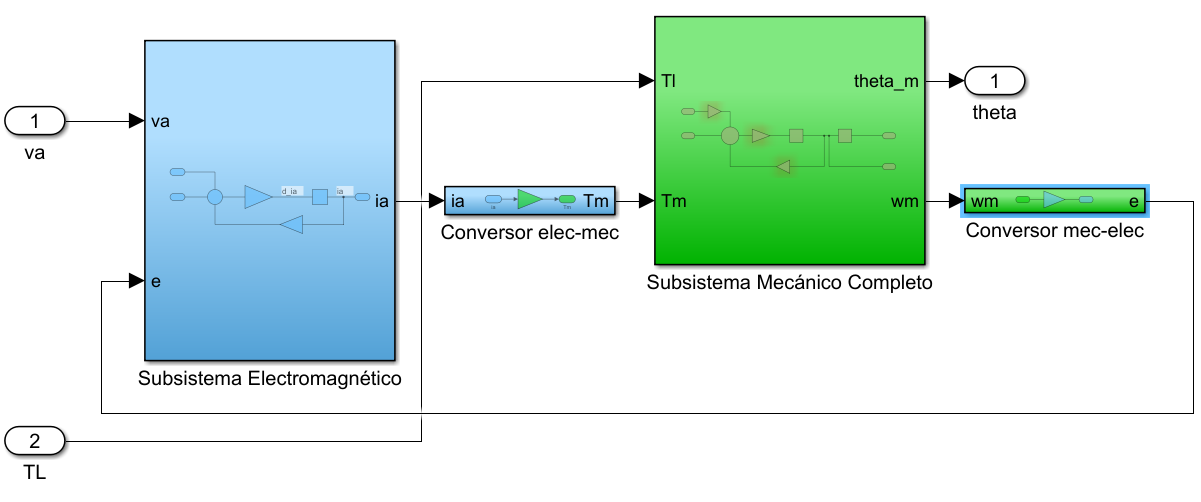
\includegraphics[width=1.1\textwidth] {Diagrama en bloques de la Planta}
    \caption{Diagrama en bloques de la Planta}
    \label{fig:Diagrama en bloques de la Planta}
\end{figure}

[[[[Dicho modelo será verificado en simulación, y luego validado comparándolo con el robot real. Aunque a falta de disponer físicamente del robot, la validación del modelo matemático propuesto a controlar se realizará comparándolo con un modelo matemático más cercano a la realidad elaborado teniendo en cuenta las no linealidades del robot]]]].



\subsubsection*{SUBSISTEMA MECÁNICO:}
\label{sec:SUBSISTEMA MECÁNICO:}

Como se explicará en el apartado controlador, el primer paso para implementar la técnica de control gain scheduling, es obtener un modelo lineal de la planta a controlar.

Para obtener el modelo matemático lineal del comportamiento no lineal de la carga mecánica del brazo robótico, se considera que
la carga posee un comportamiento lineal, mediante el uso de, en principio, los siguientes  dos parámetros equivalentes variables:
\begin{itemize}
    \item Momento de inercia equivalente (variable):
    \\ Al cambiar el ángulo de alguna otra articulación del robot, diferente a la primera, el momento de inercia respecto al eje de rotación que experimenta la primer articulación varia, y se toma como un parámetro variable.

    \item Amortiguamiento viscoso equivalente (variable):
    \\ Este amortiguamiento, corresponde a una fricción ficticia, con la cual se logra involucrar de forma equivalente los efectos de las fuerzas centrífugas y de Coriolis que aparecen cuando se mueven las demás articulaciones.
\end{itemize}

Es decir, con dichos parámetros se obtendrá un modelo lineal de parámetros variables (LPV), en donde se tiene una incertidumbre en cuál es el valor de dichos parámetros, en función de cuál es el estado dinámico de las demás articulaciones.

Aunque, debido a la simplificación de considerar un método de control monoarticular, entonces al moverse la primera articulación, la velocidad y aceleración de las demás 5 articulaciones son siempre cero. Por ello, también sus fuerzas centrífugas y de Coriolis serán siempre nulas, y por lo tanto también será siempre nulo el amortiguamiento viscoso equivalente. Es decir, que solo se necesita considerar como parámetro variable, al Momento de inercia equivalente.













\subsubsection*{Parámetros Dinámicos de los Eslabones}
\label{sec:Parámetros Dinámicos de los Eslabones}

Las empresas dedicadas a dar productos y servicios de robótica, como lo es Universal Robots, debido a la competencia del mercado no brindan al público cierta información técnica específica de sus robots, para que estos no puedan ser replicados con facilidad. Por lo que suelen ser datos que no suelen estar disponibles públicamente de forma gratuita, por propiedad de los fabricantes, ya que se los considera información técnica confidencial.

Se tuvo que realizar una extensa búsqueda, para lograr encontrar los parámetros dinámicos de los eslabones del robot UR10. La mayor dificultad se dió porque se encontraban valores que no eran coherentes con sigo mismos o bien eran de una  versión del robot distinta a la versión del modelo de la simulación en CoppeliaSim.

Para tener certeza acerca de que los valores de los parámetro dinámicos sean coherentes, se realizó el cálculo aproximado de los momentos de inercia de cada eslabón, a partir de su masa y una forma geométrica análoga simplificada utilizando las dimensiones geométricas del modelo CAD de CoppeliaSim. De esta forma, mediante prueba y error se lograron determinar cuales, de los valores de las masas y momentos de inercia de los eslabones que se disponen, son los que se corresponden correctamente con el modelo y versión del robot serie elegido para el proyecto. Dichos valores, se obtuvieron buscando información en un foro de Universal Robots, el cual posibilitó el acceso al repositorio de github: [[[https://github.com/jorgenfb/docker-ursim/blob/master/ursim-3.3.4.310/.urcontrol/urcontrol.conf.UR10]]]:


MASA DE LOS ESLABONES:
La tabla \ref{table:Masa de cada eslabón}, muestra la masa de cada eslabón en kg.
Como dato extra, la masa total del robot, la cual es igual a la suma de la masa de sus eslabónes, se ha obtenido de la hoja de datos de las epecificaciones técnicas del UR10 [[[DATASHEET]]], y es: $Mt = 28.9 kg$. Dicha masa total a sido útil para calcular la masa del eslabón base, ya que su valor no se encuentra, aunque dicha masa no es necesaria para la realización del proyecto en simulación.
\begin{table}[]
\centering
\begin{tabular}{|l|lllllll|}
\cline{1-8}
\textbf{Nombre de Eslabón}  & Base     & Hombro   & Brazo     & Codo     & Antebrazo & Muñeca   & Porta Hta. \\ \cline{1-8}
\textbf{Número del Eslabón} & 0        & 1        & 2         & 3        & 4         & 5        & 6                 \\ \cline{1-8}
\textbf{Masa del Eslabón}   & 0.465 kg & 7.100 kg & 12.700 kg & 4.270 kg & 2.000 kg  & 2.000 kg & 0.365 kg          \\ \cline{1-8}
\end{tabular}
\caption{\label{table:Masa de cada eslabón}Masa de cada eslabón.}
\end{table}
% \begin{description}
%         \item Eslabón 0:     m0 =  0.465 kg  (Base)
%         \item Eslabón 1:     m1 =  7.100 kg  (Hombro)
%         \item Eslabón 2:     m2 = 12.700 kg  (Brazo)
%         \item Eslabón 3:     m3 =  4.270 kg  (Codo)
%         \item Eslabón 4:     m4 =  2.000 kg  (Antebrazo)
%         \item Eslabón 5:     m5 =  2.000 kg  (Muñeca)
%         \item Eslabón 6:     m6 =  0.365 kg  (Porta Herramienta)
% \end{description}


MOMENTOS Y PRODUCTOS DE INERCIA:
La tabla \ref{table:Momentos y Productos de Inercia de cada eslabón}, muestra los momentos y productos de inercia, en unidades de $kg.m^2$, de cada eslabón del brazo robótico, respecto al centro de masa de cada una de ellos.
Dichos momentos y productos de inercia obtenidos del foro de universal robots tuvieron que ser reordenados, para que así coincidan con los ejes de los eslabones de robot en CoppeliaSim. % (Y además, solo a los Productos de Inercia que comenzaban con 4 decimales iguales a cero: 0.0000, los refiné a cero absoluto: 0.00000)
\begin{table}[]
\begin{center}
\begin{tabular}{l|lll|lll|l}
\cline{2-7}
& Ixx     & Iyy     & Izz     & Ixy     & Iyz      & Izx     &         \\ \cline{2-7}
Eslabón 1 & 0.03529 & 0.03408 & 0.02156 & 0.00000 & -0.00425 & 0.00000 \\
Eslabón 2 & 0.77068 & 0.76943 & 0.02814 & 0.00000 & -0.01561 & 0.00000 \\
Eslabón 3 & 0.30928 & 0.30646 & 0.01014 & 0.00000 & 0.00916  & 0.00000 \\
Eslabón 4 & 0.00296 & 0.00258 & 0.00222 & 0.00000 & -0.00024 & 0.00000 \\
Eslabón 5 & 0.00296 & 0.00222 & 0.00258 & 0.00000 & -0.00024 & 0.00000 \\
Eslabón 6 & 0.00040 & 0.00034 & 0.00041 & 0.00000 & 0.00000  & 0.00000 \\ \cline{2-7}
%             & Ixx     & Iyy     & Izz     & Ixy     & Iyz      & Izx     &                  \\ \cline{2-7}
% Eslabón 1 & 0.03529 & 0.03408 & 0.02156 & 0.00000 & -0.00425 & 0.00000 & Hombro             \\
% Eslabón 2 & 0.77068 & 0.76943 & 0.02814 & 0.00000 & -0.01561 & 0.00000 & Brazo              \\
% Eslabón 3 & 0.30928 & 0.30646 & 0.01014 & 0.00000 & 0.00916  & 0.00000 & Antebrazo          \\
% Eslabón 4 & 0.00296 & 0.00258 & 0.00222 & 0.00000 & -0.00024 & 0.00000 & Primer Mano        \\
% Eslabón 5 & 0.00296 & 0.00222 & 0.00258 & 0.00000 & -0.00024 & 0.00000 & Segunda Mano       \\
% Eslabón 6 & 0.00040 & 0.00034 & 0.00041 & 0.00000 & 0.00000  & 0.00000 & Porta Herramientas \\ \cline{2-7}
\end{tabular}
\caption{\label{table:Momentos y Productos de Inercia de cada eslabón}Momentos y Productos de Inercia de cada eslabón.}
\end{center}
\end{table}


CÁLCULO DEL MOMENTO DE INERCIA EQUIVALENTE
A continuación, se procede a obtener una fórmula matemática para el cálculo del momento de inercia equivalente respecto al ejer de giro de la primer articulación del robot. Dicho momento de inercia es variante en el tiempo, según cuál sea la posición intantantánea de las articulaciones superiores del robot, y tiene un valor mínimo y otro valor máximo los cuales son fijos y también serán calculados a continuación:


\subsubsection*{SUBSISTEMA ELECTROMAGNÉTICO:}
\label{sec:SUBSISTEMA ELECTROMAGNÉTICO:}




















% ======================================================================
\subsection{CONTROLADOR}
\label{sec:CONTROLADOR}

El controlador debe describirse con al menos las siguientes características:
\begin{enumerate}
    \item En la gran mayoría de las aplicaciones reales el controlador es digital. Por tanto, se debe modelar un controlador discreto (PID, control en espacio de estados, etc.)

    \item Si el controlador es en espacio de estados, debe agregar un observador al sistema.

    \item Se deben especificar cuáles son los objetivos del controlador. Por ejemplo, proveer estabilidad, una respuesta rápida o una respuesta subamortiguada, entre otros posibles objetivos.

    \item Se debe hacer un análisis de observabilidad.

    \item Se debe hacer un análisis de controlabilidad.

    \item Es necesario incluir un exhaustivo análisis de perturbaciones al sistema completo, el cual incluye el modelo de planta más el controlador.
\end{enumerate}

El sistema de control estará conformado por: una planta electromecánica, un controlador junto con la implementación de un observador de estados, un sensor de posición angular (encoder) y un filtro. Y el objetivo de dicho control será que el robot logre moverse sin oscilaciones, de una manera rápida y precisa, logrando brindar estabilidad y un correcto seguimiento de consignas.

El controlador que se propone es un controlador I-PD, con la idea de evitar desde un principio los problemas de amplificación de la señal de referencia que provocan la parte proporcional y derivativa, es decir, para evitar el Set-Point Kick. Esto se logra al colocar la ganancia proporcional y el bloque derivativo directamente en el lazo de realimentación, separados de la señal de referencia, como se muestra en la figura \ref{fig:Diagrama en bloques del Control (sin observador)}:

\begin{figure}[H]
    \centering
    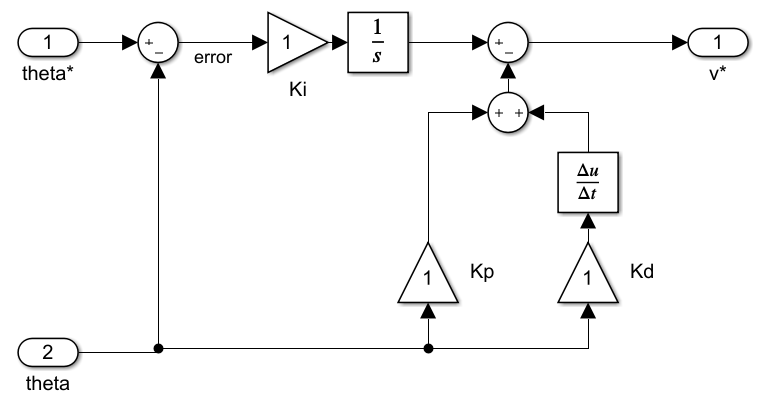
\includegraphics[width=0.60\textwidth]{Diagrama en bloques del Control (sin observador)}
    \caption{Diagrama en bloques del Control (sin observador)}
    \label{fig:Diagrama en bloques del Control (sin observador)}
\end{figure}

Como se puede ver en la figura \ref{fig:Diagrama en bloques del Control (sin observador)}, luego del bloque derivador se tiene la velocidad angular omega. Y como es conveniente no tener un bloque derivador (para evitar los problemas de amplificación de señal que conlleva la operación de derivación), se opta por eliminar este bloque derivador. Lo cual, es posible hacerlo al utilizar la variable omega estimada proveniente del observador. Es decir, que gracias a la implementación del observador, no se necesita derivar para obtener la velocidad angular. El diagrama de control quedará finalmente como se muestra en la figura \ref{fig:Diagrama en bloques del Control}.

\begin{figure}[H]
    \centering
    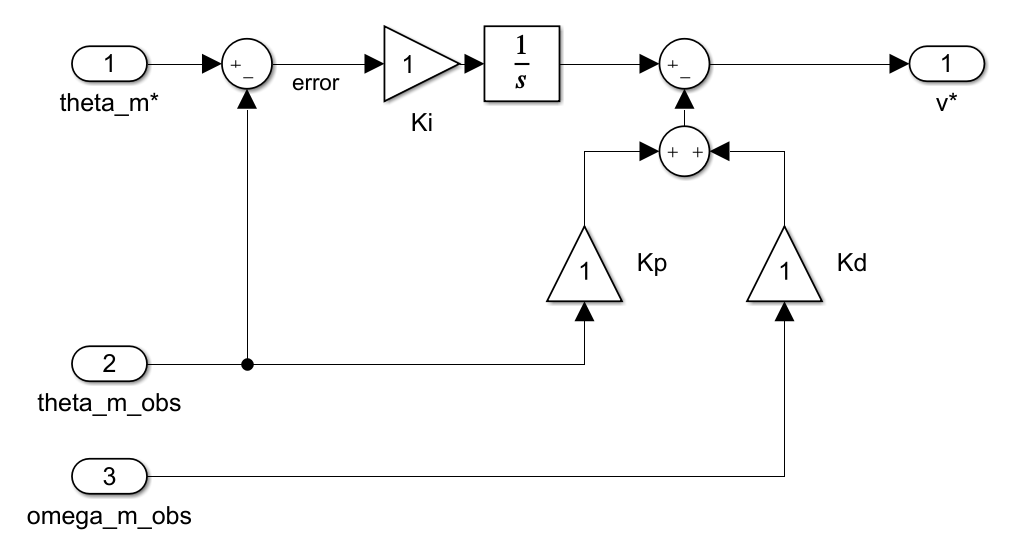
\includegraphics[width=0.60\textwidth]{Diagrama en bloques del Control}
    \caption{Diagrama en bloques del Control}
    \label{fig:Diagrama en bloques del Control}
\end{figure}

Además se modelará el sensor adicionando ruido blanco gaussiano, y se incorporará un filtro de tipo FIR en el lazo de realimentación para evitar la propagación de dicho ruido dentro del controlador.

Si resultara que el controlador I-PD porpuesto no lograra cumplir con los objetivos del proyecto, entonces se optará por un implementar alguna de las variaciones del controlador PID, como un controlador PID de dos grados de libertad.

El diagrama en bloques del sistema completo quedará como se muestra en la figura \ref{fig:Diagrama en bloques del Sistema Completo}:

\begin{figure}[H]
    \centering
    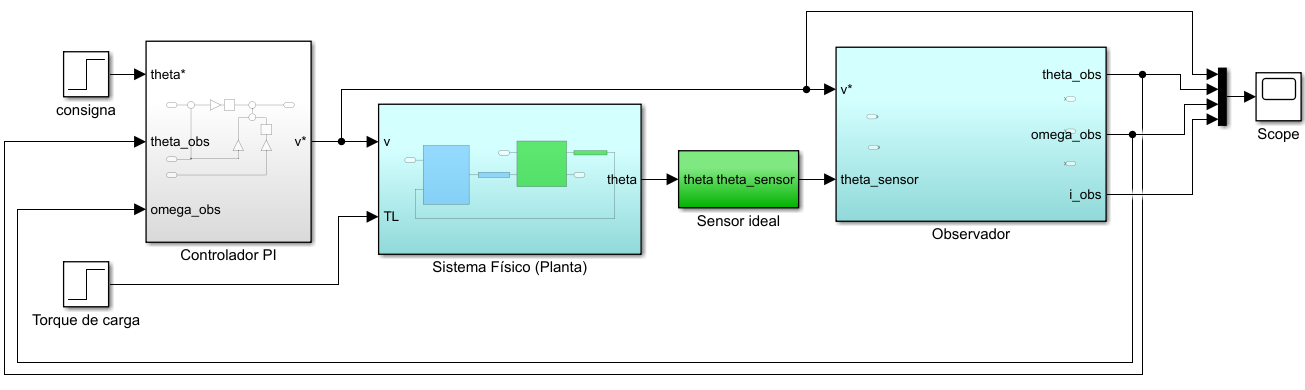
\includegraphics[width=1.1\textwidth]{Diagrama en bloques del Sistema Completo}
    \caption{Diagrama en bloques del Sistema Completo}
    \label{fig:Diagrama en bloques del Sistema Completo}
\end{figure}

El controlador se diseñará en tiempo continuo como se ha trabajado durante el cursado. Pero en la validación del modelo, el bloque del controlador será implementado en tiempo discreto con representación en punto fijo.




% ======================================================================
\subsection{PROCESAMIENTO DE SEÑALES}
\label{sec:PROCESAMIENTO DE SEÑALES}

Un sistema mecatrónico cuenta con señales de salida, las cuales son capturadas a través del uso de sensores. Dichos sensores distan de ser perfectos, por lo que siempre introducen ruido a la señal física que se trata de medir. Ejemplos de estos sensores son giróscopos, acelerómetros, encoders, sensores ultrasónicos, entre otros.

Entonces, el proyecto propuesto debe:

\begin{enumerate}

    \item Simular las imperfecciones de los sensores de salida al agregar ruido a las señales que se obtienen a la salida del modelo.

    \item La o las salidas del sistema deben ser ruidosas. El nivel de ruido debe estar en función de la hoja de datos de un sensor real.
    % \item El nivel del ruido debe replicar el de algún sensor real, según lo que conste en la hoja de datos provista por el fabricante del sensor.
\end{enumerate}






% ======================================================================
\section{RESULTADOS}
\label{sec:RESULTADOS}

Se exponen los experimentos llevados adelante. Se muestran tablas y gráficos con los valores obtenidos. Se debe dar una discusión respecto a si los resultados están dentro de los valores esperados. Se agrega al sistema una señal de perturbación y se evalúa su respuesta.


% ======================================================================
\section{CONCLUSIONES}
\label{sec:CONCLUSIONES}

Expone un resumen conciso del proyecto desarrollado y de los resultados encontrados. Se discute si se cumplió con los objetivos propuestos. Adicionalmente, se puede comentar qué aspectos del proyecto se proponen como mejora para desarrollo a futuro.

Está en \cite{masas}.






% ======================================================================
\section*{BIBLIOGRAFÍA}

Wikibooks. Online \LaTeX{} book. \href{https://en.wikibooks.org/wiki/LaTeX/}{URL}.

Overleaf. Learn LaTeX in 30 minutes. \href{https://www.overleaf.com/learn/latex/Learn_LaTeX_in_30_minutes}{URL}.

Overleaf. Bibliography management in LaTeX. \href{https://www.overleaf.com/learn/latex/Bibliography_management_in_LaTeX}{URL}.

Franco Bizzotto. Proyecto: Modelado y diseño de controlador para robot serie redundante. \href{https://github.com/carloshernangarrido/control/blob/master/12_anteproyecto_proyecto-final/Bizzotto_Robot-serie.pdf}{URL}.

Universal Robots Forum. \href{https://forum.universal-robots.com/}{URL}.

% ======================================================================
\section*{REFERENCIAS}

% @article{article,
%   author  = {Peter Adams},
%   title   = {The title of the work},
%   journal = {The name of the journal},
%   year    = 1993,
%   number  = 2,
%   pages   = {201-213},
%   month   = 7,
%   note    = {An optional note},
%   volume  = 4
% }

@misc{masas,
    author       = {Jorgen Borgesen},
    title        = {URSIM},
    howpublished = {GitHub},
    year         = 2017
}
% \href{https://github.com/jorgenfb/docker-ursim/blob/master/ursim-3.3.4.310/.urcontrol/urcontrol.conf.UR10}{https://github.com/jorgenfb/docker-ursim/blob/master/ursim-3.3.4.310/.urcontrol/urcontrol.conf.UR10}.



% ======================================================================
\section*{APÉNDICE}
% Material adicional que es importante agregar para dar un acabado entendimiento del reporte. Por ejemplo, cÓdigo fuente, planos mecÁnicos o especificaciones de sensores.

\subsection*{Código fuente en MATLAB:}
%%%%%%%%%%%%%%%%%%%%%%%%%\inputminted{matlab}{PROYECTO.m}

\subsection*{Especificaciones de Sensores:}








\bibliographystyle{ieeetr} % Estilo de citas con numeración de cada referencia.
\bibliographystyle{MiBliblioteca}
\end{document}
